
%% bare_jrnl_compsoc.tex
%% V1.4a
%% 2014/09/17
%% by Michael Shell
%% See:anastacio2006modeling
%% http://www.michaelshell.org/
%% for current contact information.
%%
%% This is a skeleton file demonstrating the use of IEEEtran.cls
%% (requires IEEEtran.cls version 1.8a or later) with an IEEE
%% Computer Society journal paper.
%%
%% Support sites:
%% http://www.michaelshell.org/tex/ieeetran/
%% http://www.ctan.org/tex-archive/macros/latex/contrib/IEEEtran/
%% and
%% http://www.ieee.org/

%%*************************************************************************
%% Legal Notice:
%% This code is offered as-is without any warranty either expressed or
%% implied; without even the implied warranty of MERCHANTABILITY or
%% FITNESS FOR A PARTICULAR PURPOSE!
%% User assumes all risk.
%% In no event shall IEEE or any contributor to this code be liable for
%% any damages or losses, including, but not limited to, incidental,
%% consequential, or any other damages, resulting from the use or misuse
%% of any information contained here.
%%
%% All comments are the opinions of their respective authors and are not
%% necessarily endorsed by the IEEE.
%%
%% This work is distributed under the LaTeX Project Public License (LPPL)
%% ( http://www.latex-project.org/ ) version 1.3, and may be freely used,
%% distributed and modified. A copy of the LPPL, version 1.3, is included
%% in the base LaTeX documentation of all distributions of LaTeX released
%% 2003/12/01 or later.
%% Retain all contribution notices and credits.
%% ** Modified files should be clearly indicated as such, including  **
%% ** renaming them and changing author support contact information. **
%%
%% File list of work: IEEEtran.cls, IEEEtran_HOWTO.pdf, bare_adv.tex,
%%                    bare_conf.tex, bare_jrnl.tex, bare_conf_compsoc.tex,
%%                    bare_jrnl_compsoc.tex, bare_jrnl_transmag.tex
%%*************************************************************************


% *** Authors should verify (and, if needed, correct) their LaTeX system  ***
% *** with the testflow diagnostic prior to trusting their LaTeX platform ***
% *** with production work. IEEE's font choices and paper sizes can       ***
% *** trigger bugs that do not appear when using other class files.       ***                          ***
% The testflow support page is at:
% http://www.michaelshell.org/tex/testflow/


\documentclass[10pt,journal,compsoc]{IEEEtran}
%
% If IEEEtran.cls has not been installed into the LaTeX system files,
% manually specify the path to it like:
% \documentclass[10pt,journal,compsoc]{../sty/IEEEtran}





% Some very useful LaTeX packages include:
% (uncomment the ones you want to load)


% *** MISC UTILITY PACKAGES ***
%
%\usepackage{ifpdf}
% Heiko Oberdiek's ifpdf.sty is very useful if you need conditional
% compilation based on whether the output is pdf or dvi.
% usage:
% \ifpdf
%   % pdf code
% \else
%   % dvi code
% \fi
% The latest version of ifpdf.sty can be obtained from:
% http://www.ctan.org/tex-archive/macros/latex/contrib/oberdiek/
% Also, note that IEEEtran.cls V1.7 and later provides a builtin
% \ifCLASSINFOpdf conditional that works the same way.
% When switching from latex to pdflatex and vice-versa, the compiler may
% have to be run twice to clear warning/error messages.






% *** CITATION PACKAGES ***
%
\ifCLASSOPTIONcompsoc
  % IEEE Computer Society needs nocompress option
  % requires cite.sty v4.0 or later (November 2003)
  \usepackage[nocompress]{cite}
\else
  % normal IEEE
  \usepackage{cite}
\fi
% cite.sty was written by Donald Arseneau
% V1.6 and later of IEEEtran pre-defines the format of the cite.sty package
% \cite{} output to follow that of IEEE. Loading the cite package will
% result in citation numbers being automatically sorted and properly
% "compressed/ranged". e.g., [1], [9], [2], [7], [5], [6] without using
% cite.sty will become [1], [2], [5]--[7], [9] using cite.sty. cite.sty's
% \cite will automatically add leading space, if needed. Use cite.sty's
% noadjust option (cite.sty V3.8 and later) if you want to turn this off
% such as if a citation ever needs to be enclosed in parenthesis.
% cite.sty is already installed on most LaTeX systems. Be sure and use
% version 5.0 (2009-03-20) and later if using hyperref.sty.
% The latest version can be obtained at:
% http://www.ctan.org/tex-archive/macros/latex/contrib/cite/
% The documentation is contained in the cite.sty file itself.
%
% Note that some packages require special options to format as the Computer
% Society requires. In particular, Computer Society  papers do not use
% compressed citation ranges as is done in typical IEEE papers
% (e.g., [1]-[4]). Instead, they list every citation separately in order
% (e.g., [1], [2], [3], [4]). To get the latter we need to load the cite
% package with the nocompress option which is supported by cite.sty v4.0
% and later. Note also the use of a CLASSOPTION conditional provided by
% IEEEtran.cls V1.7 and later.





% *** GRAPHICS RELATED PACKAGES ***
%
\ifCLASSINFOpdf
  % \usepackage[pdftex]{graphicx}
  % declare the path(s) where your graphic files are
  % \graphicspath{{../pdf/}{../jpeg/}}
  % and their extensions so you won't have to specify these with
  % every instance of \includegraphics
  % \DeclareGraphicsExtensions{.pdf,.jpeg,.png}
\else
  % or other class option (dvipsone, dvipdf, if not using dvips). graphicx
  % will default to the driver specified in the system graphics.cfg if no
  % driver is specified.
  % \usepackage[dvips]{graphicx}
  % declare the path(s) where your graphic files are
  % \graphicspath{{../eps/}}
  % and their extensions so you won't have to specify these with
  % every instance of \includegraphics
  % \DeclareGraphicsExtensions{.eps}
\fi
% graphicx was written by David Carlisle and Sebastian Rahtz. It is
% required if you want graphics, photos, etc. graphicx.sty is already
% installed on most LaTeX systems. The latest version and documentation
% can be obtained at:
% http://www.ctan.org/tex-archive/macros/latex/required/graphics/
% Another good source of documentation is "Using Imported Graphics in
% LaTeX2e" by Keith Reckdahl which can be found at:
% http://www.ctan.org/tex-archive/info/epslatex/
%
% latex, and pdflatex in dvi mode, support graphics in encapsulated
% postscript (.eps) format. pdflatex in pdf mode supports graphics
% in .pdf, .jpeg, .png and .mps (metapost) formats. Users should ensure
% that all non-photo figures use a vector format (.eps, .pdf, .mps) and
% not a bitmapped formats (.jpeg, .png). IEEE frowns on bitmapped formats
% which can result in "jaggedy"/blurry rendering of lines and letters as
% well as large increases in file sizes.
%
% You can find documentation about the pdfTeX application at:
% http://www.tug.org/applications/pdftex






% *** MATH PACKAGES ***
%
%\usepackage[cmex10]{amsmath}
% A popular package from the American Mathematical Society that provides
% many useful and powerful commands for dealing with mathematics. If using
% it, be sure to load this package with the cmex10 option to ensure that
% only type 1 fonts will utilized at all point sizes. Without this option,
% it is possible that some math symbols, particularly those within
% footnotes, will be rendered in bitmap form which will result in a
% document that can not be IEEE Xplore compliant!
%
% Also, note that the amsmath package sets \interdisplaylinepenalty to 10000
% thus preventing page breaks from occurring within multiline equations. Use:
%\interdisplaylinepenalty=2500
% after loading amsmath to restore such page breaks as IEEEtran.cls normally
% does. amsmath.sty is already installed on most LaTeX systems. The latest
% version and documentation can be obtained at:
% http://www.ctan.org/tex-archive/macros/latex/required/amslatex/math/





% *** SPECIALIZED LIST PACKAGES ***
%
%\usepackage{algorithmic}
% algorithmic.sty was written by Peter Williams and Rogerio Brito.
% This package provides an algorithmic environment fo describing algorithms.
% You can use the algorithmic environment in-text or within a figure
% environment to provide for a floating algorithm. Do NOT use the algorithm
% floating environment provided by algorithm.sty (by the same authors) or
% algorithm2e.sty (by Christophe Fiorio) as IEEE does not use dedicated
% algorithm float types and packages that provide these will not provide
% correct IEEE style captions. The latest version and documentation of
% algorithmic.sty can be obtained at:
% http://www.ctan.org/tex-archive/macros/latex/contrib/algorithms/
% There is also a support site at:
% http://algorithms.berlios.de/index.html
% Also of interest may be the (relatively newer and more customizable)
% algorithmicx.sty package by Szasz Janos:
% http://www.ctan.org/tex-archive/macros/latex/contrib/algorithmicx/




% *** ALIGNMENT PACKAGES ***
%
%\usepackage{array}
% Frank Mittelbach's and David Carlisle's array.sty patches and improves
% the standard LaTeX2e array and tabular environments to provide better
% appearance and additional user controls. As the default LaTeX2e table
% generation code is lacking to the point of almost being broken with
% respect to the quality of the end results, all users are strongly
% advised to use an enhanced (at the very least that provided by array.sty)
% set of table tools. array.sty is already installed on most systems. The
% latest version and documentation can be obtained at:
% http://www.ctan.org/tex-archive/macros/latex/required/tools/


% IEEEtran contains the IEEEeqnarray family of commands that can be used to
% generate multiline equations as well as matrices, tables, etc., of high
% quality.




% *** SUBFIGURE PACKAGES ***
%\ifCLASSOPTIONcompsoc
%  \usepackage[caption=false,font=footnotesize,labelfont=sf,textfont=sf]{subfig}
%\else
%  \usepackage[caption=false,font=footnotesize]{subfig}
%\fi
% subfig.sty, written by Steven Douglas Cochran, is the modern replacement
% for subfigure.sty, the latter of which is no longer maintained and is
% incompatible with some LaTeX packages including fixltx2e. However,
% subfig.sty requires and automatically loads Axel Sommerfeldt's caption.sty
% which will override IEEEtran.cls' handling of captions and this will result
% in non-IEEE style figure/table captions. To prevent this problem, be sure
% and invoke subfig.sty's "caption=false" package option (available since
% subfig.sty version 1.3, 2005/06/28) as this is will preserve IEEEtran.cls
% handling of captions.
% Note that the Computer Society format requires a sans serif font rather
% than the serif font used in traditional IEEE formatting and thus the need
% to invoke different subfig.sty package options depending on whether
% compsoc mode has been enabled.
%
% The latest version and documentation of subfig.sty can be obtained at:
% http://www.ctan.org/tex-archive/macros/latex/contrib/subfig/




% *** FLOAT PACKAGES ***
%
%\usepackage{fixltx2e}
% fixltx2e, the successor to the earlier fix2col.sty, was written by
% Frank Mittelbach and David Carlisle. This package corrects a few problems
% in the LaTeX2e kernel, the most notable of which is that in current
% LaTeX2e releases, the ordering of single and double column floats is not
% guaranteed to be preserved. Thus, an unpatched LaTeX2e can allow a
% single column figure to be placed prior to an earlier double column
% figure. The latest version and documentation can be found at:
% http://www.ctan.org/tex-archive/macros/latex/base/


%\usepackage{stfloats}
% stfloats.sty was written by Sigitas Tolusis. This package gives LaTeX2e
% the ability to do double column floats at the bottom of the page as well
% as the top. (e.g., "\begin{figure*}[!b]" is not normally possible in
% LaTeX2e). It also provides a command:
%\fnbelowfloat
% to enable the placement of footnotes below bottom floats (the standard
% LaTeX2e kernel puts them above bottom floats). This is an invasive package
% which rewrites many portions of the LaTeX2e float routines. It may not work
% with other packages that modify the LaTeX2e float routines. The latest
% version and documentation can be obtained at:
% http://www.ctan.org/tex-archive/macros/latex/contrib/sttools/
% Do not use the stfloats baselinefloat ability as IEEE does not allow
% \baselineskip to stretch. Authors submitting work to the IEEE should note
% that IEEE rarely uses double column equations and that authors should try
% to avoid such use. Do not be tempted to use the cuted.sty or midfloat.sty
% packages (also by Sigitas Tolusis) as IEEE does not format its papers in
% such ways.
% Do not attempt to use stfloats with fixltx2e as they are incompatible.
% Instead, use Morten Hogholm'a dblfloatfix which combines the features
% of both fixltx2e and stfloats:
%
% \usepackage{dblfloatfix}
% The latest version can be found at:
% http://www.ctan.org/tex-archive/macros/latex/contrib/dblfloatfix/




%\ifCLASSOPTIONcaptionsoff
%  \usepackage[nomarkers]{endfloat}
% \let\MYoriglatexcaption\caption
% \renewcommand{\caption}[2][\relax]{\MYoriglatexcaption[#2]{#2}}
%\fi
% endfloat.sty was written by James Darrell McCauley, Jeff Goldberg and
% Axel Sommerfeldt. This package may be useful when used in conjunction with
% IEEEtran.cls'  captionsoff option. Some IEEE journals/societies require that
% submissions have lists of figures/tables at the end of the paper and that
% figures/tables without any captions are placed on a page by themselves at
% the end of the document. If needed, the draftcls IEEEtran class option or
% \CLASSINPUTbaselinestretch interface can be used to increase the line
% spacing as well. Be sure and use the nomarkers option of endfloat to
% prevent endfloat from "marking" where the figures would have been placed
% in the text. The two hack lines of code above are a slight modification of
% that suggested by in the endfloat docs (section 8.4.1) to ensure that
% the full captions always appear in the list of figures/tables - even if
% the user used the short optional argument of \caption[]{}.
% IEEE papers do not typically make use of \caption[]'s optional argument,
% so this should not be an issue. A similar trick can be used to disable
% captions of packages such as subfig.sty that lack options to turn off
% the subcaptions:
% For subfig.sty:
% \let\MYorigsubfloat\subfloat
% \renewcommand{\subfloat}[2][\relax]{\MYorigsubfloat[]{#2}}
% However, the above trick will not work if both optional arguments of
% the \subfloat command are used. Furthermore, there needs to be a
% description of each subfigure *somewhere* and endfloat does not add
% subfigure captions to its list of figures. Thus, the best approach is to
% avoid the use of subfigure captions (many IEEE journals avoid them anyway)
% and instead reference/explain all the subfigures within the main caption.
% The latest version of endfloat.sty and its documentation can obtained at:
% http://www.ctan.org/tex-archive/macros/latex/contrib/endfloat/
%
% The IEEEtran \ifCLASSOPTIONcaptionsoff conditional can also be used
% later in the document, say, to conditionally put the References on a
% page by themselves.




% *** PDF, URL AND HYPERLINK PACKAGES ***
%
%\usepackage{url}
% url.sty was written by Donald Arseneau. It provides better support for
% handling and breaking URLs. url.sty is already installed on most LaTeX
% systems. The latest version and documentation can be obtained at:
% http://www.ctan.org/tex-archive/macros/latex/contrib/url/
% Basically, \url{my_url_here}.





% *** Do not adjust lengths that control margins, column widths, etc. ***
% *** Do not use packages that alter fonts (such as pslatex).         ***
% There should be no need to do such things with IEEEtran.cls V1.6 and later.
% (Unless specifically asked to do so by the journal or conference you plan
% to submit to, of course. )

%Mine
\usepackage{graphicx}
\usepackage{caption}
\usepackage{subcaption}
\usepackage{algorithm}
\usepackage{algorithmicx}
\usepackage{algpseudocode}
\usepackage{amsmath}

% correct bad hyphenation here
\hyphenation{op-tical net-works semi-conduc-tor}


\begin{document}



%
% paper title
% Titles are generally capitalized except for words such as a, an, and, as,
% at, but, by, for, in, nor, of, on, or, the, to and up, which are usually
% not capitalized unless they are the first or last word of the title.
% Linebreaks \\ can be used within to get better formatting as desired.
% Do not put math or special symbols in the title.
\title{Capturing, Rendering and Simulation for Large Scale Grassland}
%
%
% author names and IEEE memberships
% note positions of commas and nonbreaking spaces ( ~ ) LaTeX will not break
% a structure at a ~ so this keeps an author's name from being broken across
% two lines.
% use \thanks{} to gain access to the first footnote area
% a separate \thanks must be used for each paragraph as LaTeX2e's \thanks
% was not built to handle multiple paragraphs
%
%
%\IEEEcompsocitemizethanks is a special \thanks that produces the bulleted
% lists the Computer Society journals use for "first footnote" author
% affiliations. Use \IEEEcompsocthanksitem which works much like \item
% for each affiliation group. When not in compsoc mode,
% \IEEEcompsocitemizethanks becomes like \thanks and
% \IEEEcompsocthanksitem becomes a line break with idention. This
% facilitates dual compilation, although admittedly the differences in the
% desired content of \author between the different types of papers makes a
% one-size-fits-all approach a daunting prospect. For instance, compsoc
% journal papers have the author affiliations above the "Manuscript
% received ..."  text while in non-compsoc journals this is reversed. Sigh.

\author{
Zengzhi Fan, Shanghai Jiao Tong University

Bin Sheng, Shanghai Jiao Tong University
\IEEEcompsocitemizethanks{\IEEEcompsocthanksitem B.Sheng is with the Department
of Computer Science and Engineering, Shanghai Jiao Tong, Shanghai,
China, 200240.\protect\\
% note need leading \protect in front of \\ to get a newline within \thanks as
% \\ is fragile and will error, could use \hfil\break instead.
E-mail: shengbin@cs.sjtu.edu.cn}


}

% note the % following the last \IEEEmembership and also \thanks -
% these prevent an unwanted space from occurring between the last author name
% and the end of the author line. i.e., if you had this:
%
% \author{....lastname \thanks{...} \thanks{...} }
%                     ^------------^------------^----Do not want these spaces!
%
% a space would be appended to the last name and could cause every name on that
% line to be shifted left slightly. This is one of those "LaTeX things". For
% instance, "\textbf{A} \textbf{B}" will typeset as "A B" not "AB". To get
% "AB" then you have to do: "\textbf{A}\textbf{B}"
% \thanks is no different in this regard, so shield the last } of each \thanks
% that ends a line with a % and do not let a space in before the next \thanks.
% Spaces after \IEEEmembership other than the last one are OK (and needed) as
% you are supposed to have spaces between the names. For what it is worth,
% this is a minor point as most people would not even notice if the said evil
% space somehow managed to creep in.



% The paper headers
\markboth{Journal of \LaTeX\ Class Files,~Vol.~13, No.~9, September~2014}%
{Shell \MakeLowercase{\textit{et al.}}: Bare Demo of IEEEtran.cls for Computer Society Journals}
% The only time the second header will appear is for the odd numbered pages
% after the title page when using the twoside option.
%
% *** Note that you probably will NOT want to include the author's ***
% *** name in the headers of peer review papers.                   ***
% You can use \ifCLASSOPTIONpeerreview for conditional compilation here if
% you desire.



% The publisher's ID mark at the bottom of the page is less important with
% Computer Society journal papers as those publications place the marks
% outside of the main text columns and, therefore, unlike regular IEEE
% journals, the available text space is not reduced by their presence.
% If you want to put a publisher's ID mark on the page you can do it like
% this:
%\IEEEpubid{0000--0000/00\$00.00~\copyright~2014 IEEE}
% or like this to get the Computer Society new two part style.
%\IEEEpubid{\makebox[\columnwidth]{\hfill 0000--0000/00/\$00.00~\copyright~2014 IEEE}%
%\hspace{\columnsep}\makebox[\columnwidth]{Published by the IEEE Computer Society\hfill}}
% Remember, if you use this you must call \IEEEpubidadjcol in the second
% column for its text to clear the IEEEpubid mark (Computer Society jorunal
% papers don't need this extra clearance.)



% use for special paper notices
%\IEEEspecialpapernotice{(Invited Paper)}


% for Computer Society papers, we must declare the abstract and index terms
% PRIOR to the title within the \IEEEtitleabstractindextext IEEEtran
% command as these need to go into the title area created by \maketitle.
% As a general rule, do not put math, special symbols or citations
% in the abstract or keywords.
\IEEEtitleabstractindextext{%
\begin{abstract}
Grass is a very import element of nature, however creating, rendering and simulating a large scale grassland is not easy due to extremely high computation complexity and large amount of data needed for simulation and rendering. Grass modeling does not usually draw enough attention due to its simple structure while it still remains a problem to set up a proper grass blade model for rendering and simulation. Moreover there are numerous categories of grass blades in this world and it's not possible for any system to store all kinds of grass blades in advance. Capturing grass blade with interactive camera can be an intuitive solution for this problem. We provide a method that can capture grass blade shapes with a depth camera, render large scale grassland efficiently and simulate this grassland with individual response for each single blade on the fly. 
\end{abstract}

% Note that keywords are not normally used for peerreview papers.
\begin{IEEEkeywords}
Grass, Capture, Render, Simulation, GPU
\end{IEEEkeywords}}

 %% Uncomment below to include a teaser figure.
 %% Note: No figures other than the optional teaser are permitted on title page.


% make the title area
%\maketitle

\twocolumn[{%
\renewcommand\twocolumn[1][]{#1}%
\maketitle
\begin{center}
    \centering
    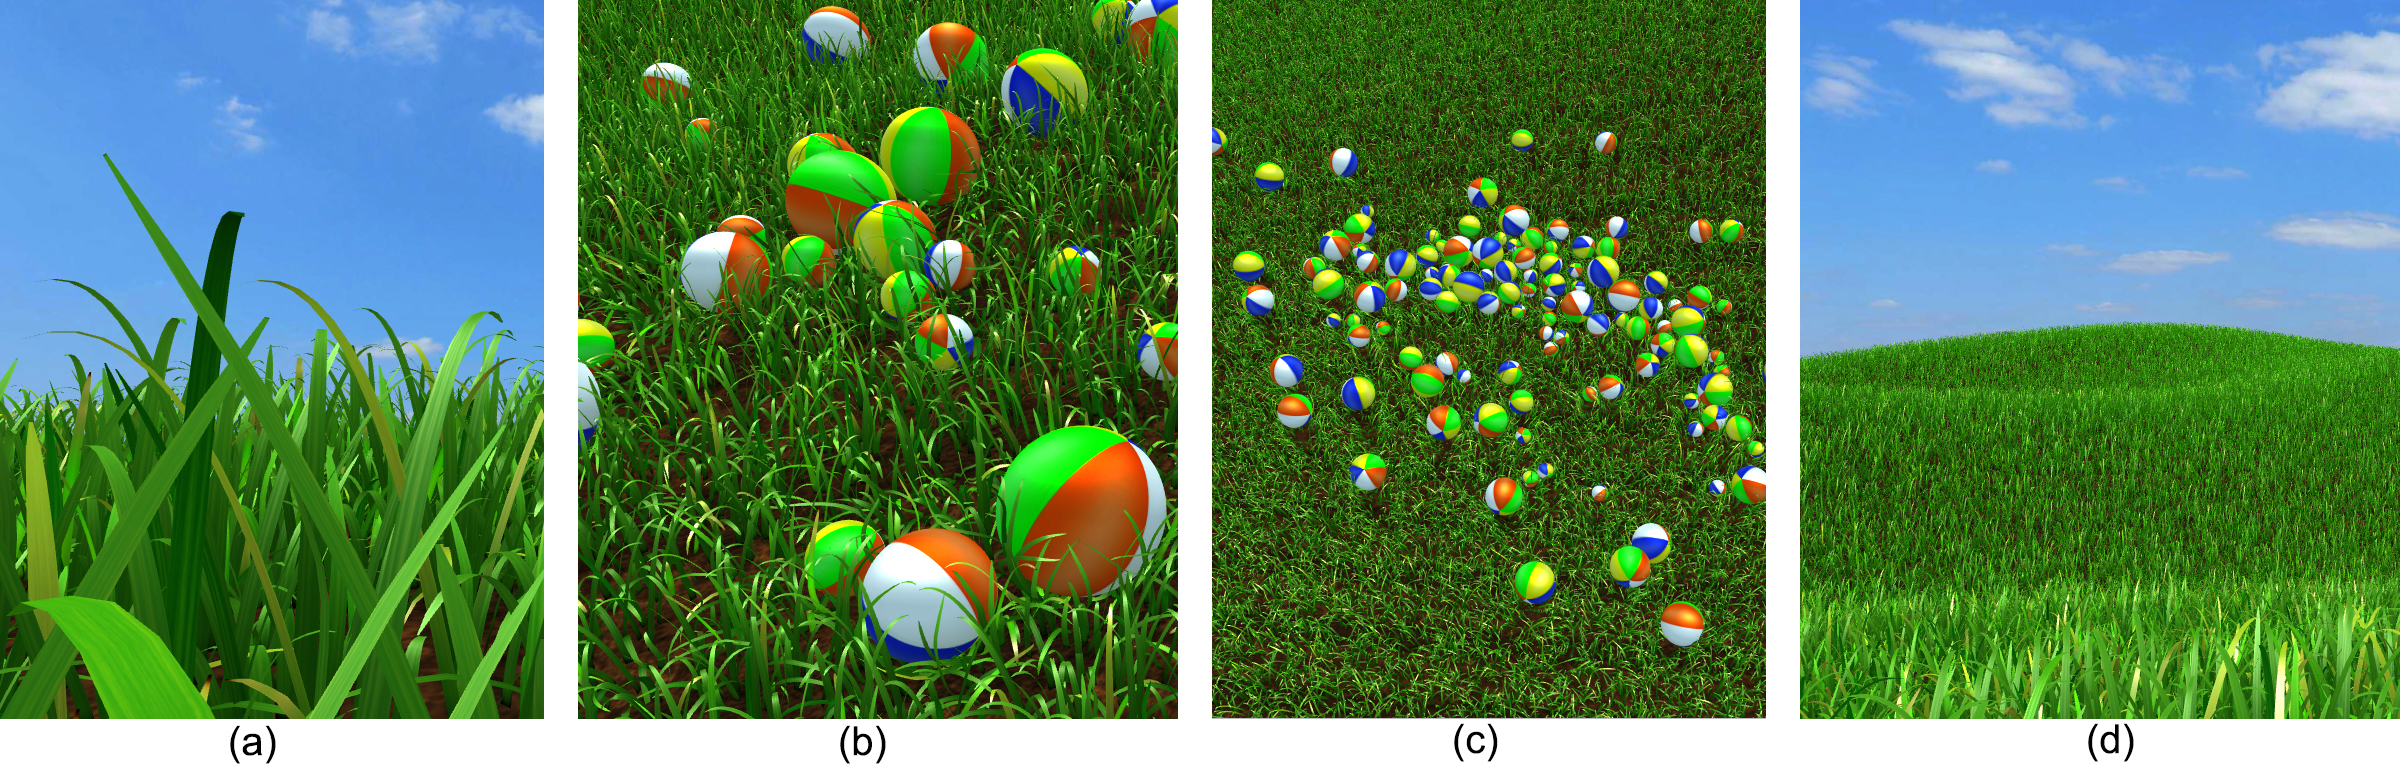
\includegraphics[width=1.0\textwidth]{figs/teaser.jpg}
    \captionof{figure}{Large scale grassland with our method: (a) grass detail in the scene; (b) front view of large scale grassland in test scene.\\\\
    }
    \label{fig:teaser}
\end{center}%
}]



% To allow for easy dual compilation without having to reenter the
% abstract/keywords data, the \IEEEtitleabstractindextext text will
% not be used in maketitle, but will appear (i.e., to be "transported")
% here as \IEEEdisplaynontitleabstractindextext when the compsoc
% or transmag modes are not selected <OR> if conference mode is selected
% - because all conference papers position the abstract like regular
% papers do.
\IEEEdisplaynontitleabstractindextext
% \IEEEdisplaynontitleabstractindextext has no effect when using
% compsoc or transmag under a non-conference mode.



% For peer review papers, you can put extra information on the cover
% page as needed:
% \ifCLASSOPTIONpeerreview
% \begin{center} \bfseries EDICS Category: 3-BBND \end{center}
% \fi
%
% For peerreview papers, this IEEEtran command inserts a page break and
% creates the second title. It will be ignored for other modes.
\IEEEpeerreviewmaketitle



\IEEEraisesectionheading{\section{Introduction}\label{sec:introduction}}
% Computer Society journal (but not conference!) papers do something unusual
% with the very first section heading (almost always called "Introduction").
% They place it ABOVE the main text! IEEEtran.cls does not automatically do
% this for you, but you can achieve this effect with the provided
% \IEEEraisesectionheading{} command. Note the need to keep any \label that
% is to refer to the section immediately after \section in the above as
% \IEEEraisesectionheading puts \section within a raised box.

\IEEEPARstart{G}{rass} is a significant feature of natural world and it is indispensable in most 3D games and movies .Therefore the modeling, rendering and simulation of grass become an essential field of computer graphics and visualization. When an object passes on a grassland, every grass blade on the path is pushed aside or run over, and gradually recovers its shape afterwards. Individual responses from every single grass blade greatly improve viewers' experience for virtual environment and increase scene's fidelity. Realistic modeling for grass blade rendering is not easy since grass blade shape varies a lot. Artists usually disregard the importance of grass blades modeling for their simple structure, meanwhile the lack of realistic grass blade model becomes a frequent issue when creating virtual scenes for games and other 3D applications.\\

Grass modeling, rendering and simulation may not be so difficult for a single blade, however challenge comes when quantity is taken into consideration. Geometry-based modeling is used in most methods where structures are represented as triangles. Nevertheless when there is requirement for large quantity of grass blades, vertex amount for a single grass blade is strictly limited to a very small number for the sake of high performance. Modeling realistic grass blade with vertex amount restriction is challenging, no mater manually or recovering from images or videos. Compared with hair, which could be described with line segments, grass blade has far more kinds of shapes and structures meanwhile there are even more grass blades required for rendering and simulation than hairs in most cases. Therefore current hair rendering techniques are not applicable for scenes with extreme large amount of grass blades and various grass shapes. Simulation for hair is rather a group problem since movements for hairs are quite similar. Thus hairs can be divided into groups and guide hairs are usually used as representatives for simulation. Head movement is the major cause of hair movement and head movement range is rather small and highly predictable, which greatly reduces the difficulty of hair simulation. For grass blades, individual response for any other objects is essential and cannot be simply divided into groups for simulation. This becomes the key problem for grass simulation. Besides, grass blades have stationary shapes, they should recover their shapes and positions after collision.\\

In this paper we present a novel and effective framework for extremely large amount of grass blades modeling, rendering and simulation. Our framework is able to capture grass blade from camera, refine grass blade shape and render large scale grassland scene with high quality as well as realistic simulation response to collisions. Depth cameras are specially valued since they are able to provide depth information of any scene, which makes it much easier to rebuild any object or scene. With depth camera, we are able to capture grass blade shape instantly instead of using a small number of preset shapes. Compared with image-based method, depth-camera-based method is much faster and is able to get far more accurate depth information. More importantly, cameras provide human-computer interaction and allow users to adjust capturing results through instant feedback on the screen. Camera-based method also provide possibility for inexperienced users to create models for their own virtual scenes.\\

In order to deal with extremely large grass blade amount and achieve real-time performance of rendering and simulation, triangles are abandoned for grass representation. Grass blades are stored as line segments and are expanded to their final shape at run time. Line segments are extracted from depth image as grass blade skeleton meanwhile expansion width for each vertex is calculated from blades' contour obtained from depth camera. Expansion widths partially define blades' shape and structure. A particle-flow method is adopted to partition single blade contour from a cluster blades. \\

In our system every single grass blade has individual and realistic response to collision. We apply GPU-based instancing to lower the requirement for memory and bandwidth, and pay simulation costs only when needed. Meanwhile, this is a tile-based rendering and simulation system, no per-tile data is store unless simulation for a specific tile is required. We implement the method introduced by Han et al.\cite{han2012real} to simulate our grass blade and extend the method introduced by Fan et al.\cite{fan2015simulation} to do tile management. Unlike any simulation only for key blades or hairs in the scene, each grass blade could have separate movement and independent collision to objects. Real-time performance is achieved with more than one million grass blades and hundreds of objects.

Our main contributions are listed below:
\begin{itemize}
\item Interactive grass blade capturing method with depth camera,including skeleton extraction and expansion width calculation;
\item Blade skeleton simplification and refinement according to vertices' movement similarity;
\item Extension for large scale grassland rendering as well as simulation method with high fidelity, which allow instant shape editing during rendering and simulation.
\end{itemize}

% needed in second column of first page if using \IEEEpubid
%\IEEEpubidadjcol

\section{Related Work}
The most challenging part of grass modeling, rendering and simulation is caused by extremely large quantity. William Reeves and Ricki Blau\cite{reeves1985approximate} addressed those challenges in 1985. Works about grass mainly discuss the following three topics: grass modeling, rendering and simulation.  Kajiya et al.\cite{kajiya1989rendering} introduced volumetric textures(texels) for short fur rendering. Texels can used to solve spatial aliasing problem. Neyret extended this work to simulate natural scenes such as realistic grass\cite{neyret1996synthesizing} \cite{neyret1998modeling}. Polygons stacks as well as semi-transparent textures were used in implementation of texels\cite{meyer1998interactive}. Brook et al\cite{bakay2002real} improved this method to obtain high rendering performance. Image-based method was used in grass rendering\cite{shah2005real}. This method used bidirectional texture function for grass. Boulanger et al.\cite{boulanger2009rendering} introduced a level-of-detail(LOD) method for grass rendering with realistic dynamic light and shadow effects. In previous works, grass blades were pushed away when interaction between grass blades and objects happens\cite{guerraz2003procedural}. Spring-mass system was also used to model grass blade and simulate grass-object interaction\cite{chen2010real}\cite{hempe2013generation}. A method to modeling withering grass was introduced by Wen et al.\cite{wu2012using} using time-varying texels. We adopt the simulation algorithm introduced by Han et al.\cite{han2012real}. This method treated collision as hard constraint, meanwhile treated length, bending and twisting as soft constraints in the iterative solver for grass-object interaction. We employ the rendering and simulation framework introduced by \cite{fan2015simulation}. With this frame work, we are able to perform collision computation on GPU and do grass blade instancing on the fly.  We implement our capture method on the basis of this framework to obtain more accurate and diverse grass types.\\

A number of works for leaf and flora reconstruction have reference value for our method. There are some previous works about using interactive method to generate or reconstruct leaf shapes and tree shapes\cite{mundermann2003modeling}\cite{okabe2005interactive}\cite{anastacio2006modeling}\cite{chen2008sketch}\cite{pirk2012plastic}.Quan et al.\cite{quan2006image} introduced a method to model plant from a dozen of images. This method could recover plant's shape automatically while relying on user to provide some hints for segmentation. Tan et al.\cite{tan2007image} proposed a method to generate 3D trees from images. They populated tree leaves from segmented source images and used shape patterns of visible branches to predict occluded branches. Tree modeling from single image was introduced afterwards\cite{tan2008single}. Yan et al.\cite{yan2014flower} came up with a method for flower reconstruction from a single image, which used a cone fitting scheme to maintains flower shape.Bradley et al.\cite{bradley2013image} presented a scale technique to compute 3D structure of foliage and extract leaf shapes.\\

Capturing grass blade with camera has not been explored much, however plenty of researches about hair capture have been conducted. There are some similarities between hair and grass blade for their shapes and movement features. Chai et al.\cite{chai2012single} uses single image to do hair modeling, they captured hair style from image and were able to render origin hair style at different angle, with different hair materials and change hair style . Afterwards, they extended their work through user's high-level knowledge to get more accurate hair that matches image and waa physically real at the same time. By doing it they were able to finish dynamic hair simulation and interactive hair style editing, which made it possible to apply this hair manipulation in video\cite{chai2013dynamic}. A structure-aware hair capture method\cite{luo2013structure} was introduced in 2013, authors adopted a method to generate hair strand segments, set up a connection graph to guarantee hair growth to areas with missed geometry information and connected hair strands with consistent curvature. A method to capture hair using simulated examples was introduced by Hu et al.\cite{hu2014robust}, they used simulated samples as references to generate hair, and this method could be applied with unconstrained and constrained hair. They also came up with a method to capture braided hair style\cite{hu2014capturing}. A data-driven reconstruction method was adopted in this scheme and procedurally generated examples were used to fit captured hair strands. Xu et al.\cite{xu2014dynamic} introduced a space-time optimization method to capture dynamic hair. This method could faithfully capture hair strands' shape as well as spatial details.\\

Level-of-detail(LOD) methods are typical model simplification algorithms, they are used to simplify model geometry complexity and accelerate rendering as well as simulation performance. Framework used to obtain a constant frame rate for visualization of virtual environments was introduced in 1993\cite{funkhouser1993adaptive}. Geometry-based LOD algorithms including quad remeshing methods were summarized in \cite{bommes2013quad}. Field-guided parameterization-based methods split quad remeshing into three steps including cross-field computation, integer-grid parameterization and quad mesh extraction\cite{ray2006periodic}\cite{kalberer2007quadcover}
\cite{bommes2009mixed}\cite{zhang2010wave}. Except for those geometry-based LOD algorithms, level-of-detail was also used in simulation method. Techniques for reducing the computational complexity for simulations was introduced by Carlson et al.\cite{simulation1997Deborah}. LOD was also used for animation and rendering of prairies and particle systems\cite{o2001automatic}. Our skeleton refining method is similar to those LOD algorithms, moreover we take simulation fidelity into account while simplifying grass blade model. This leads to more accurate model for rendering and simulation at the same time and we are able to balance the trade-off between performance and quality.\\

\section{Algorithm Overview}


\begin{figure*}
    \centering
    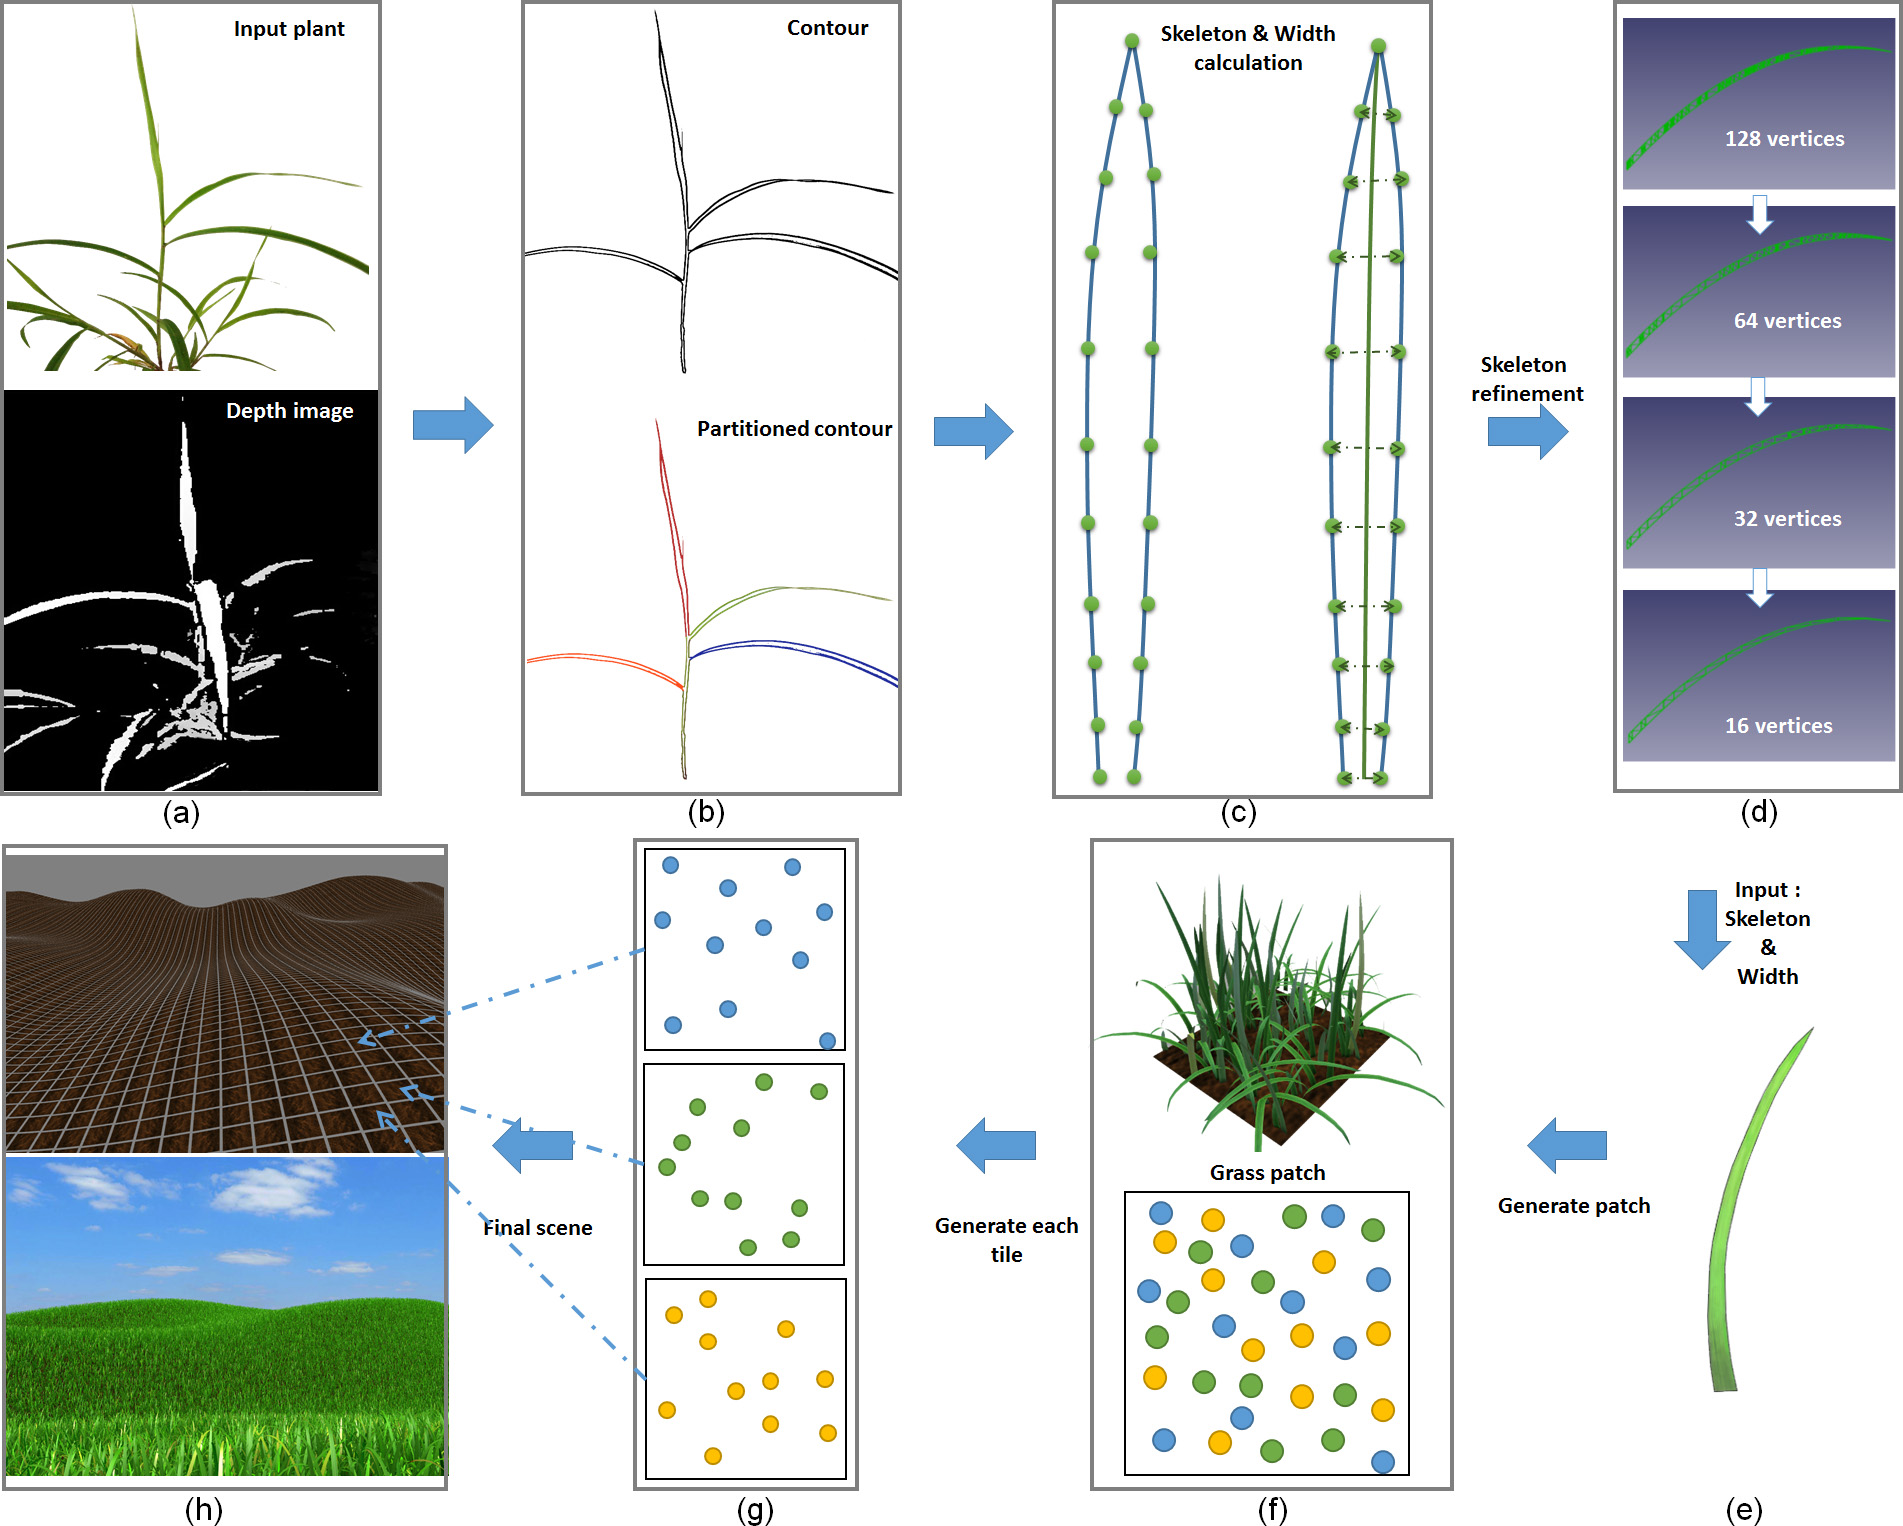
\includegraphics[width=1.0\textwidth]{figs/overview.jpg}
    \captionof{figure}{Overview of system pipeline:(a) a cluster of grass blades and depth depth image captured with camera, those are raw data in our system; (b) extracted contour(top), partitioned contour for a single blade marked with different color respectively(bottom);(c) skeleton and expansion width calculation; (d) skeleton refining process with a initial blade skeleton with 128 vertices, skeleton vertices are reduced down to 64,32 and 16 with different refining levels ; (e) input skeleton and expansion width that could describe the grass blade; (f) instancing scheme:using refined skeleton to generate a grass patch, randomize grass blades' length, orientation and location in a tile; (g) every tile refer to a subset of grass blades in the patch; (h) expand skeleton to grass according to expansion width at run time, render the whole scene and do simulation.}
    \label{fig:overview}
\end{figure*}

The overview of our algorithm is shown in Figure.\ref{fig:overview}. We employ a depth camera in our system which is able to obtain depth image of target plant. According to this depth image, we are able to extract the contour of grass blades by distance masking method in real time, which is difficult to achieve without depth information. Single blade's contour could be partitioned from a cluster of blades by a particle-flow method\cite{neubert2007approximate}.\\

According to contour of grass blade, we calculate blade's skeleton, which is used to describe this blade and is also used in simulation. In vertex shader we expand each knot on the skeleton to form the blade. Expansion widths are calculated from blade's contour and smoothed before rendering.\\

For skeleton captured from camera, we design an refining algorithm to do simplification. This process is similar to level-of-detail(LOD). Since skeleton knots number is restricted by extremely large amount of grass blades, this refining algorithm could reduce skeleton knots number from over one hundred to $32$, $16$ or even less, according to knots' movement similarity.\\

We adopt the GPU instancing scheme used in \cite{fan2015simulation}. We pre-generate a list of grass blade called grass patch. Grass scene is divided into a grid of tiles. Grass blades in each tile are specific number of continuous blades fetched from grass patch. Starting position in grass patch for each tile is calculated by tile's position in the scene. Blade's skeleton is expanded to triangles before rendering. Phong shading model is used in grass blade rendering for the sake of high performance. Subsurface scattering effects is also used in our system to increase fidelity\cite{sousa2007vegetation}. Tile management guarantee per-blade memory is allocated only when simulation is needed.  \\

\section{Algorithm Details}\label{sec:detail}
\subsection{Blade Capture}\label{sec:capture}
we aim to capture grass blade without manual operations and use capture result in the rendering and simulation system immediately after capturing. Skeleton knots number limits the detail level of our grass blade, however it also requires efficient refining algorithm to convert captured skeleton into appropriate blade model in our system. Motivated by other hair and plant capture methods, we adopt a depth camera to capture grass blade. Depth cameras are deployed in variety of applications and becoming prevailing more than ever, for its advantage to recover shapes and capture movements. With depth camera, we manage to capture grass blade and mask non-grass object on the fly.\\

\begin{figure}
    \centering
    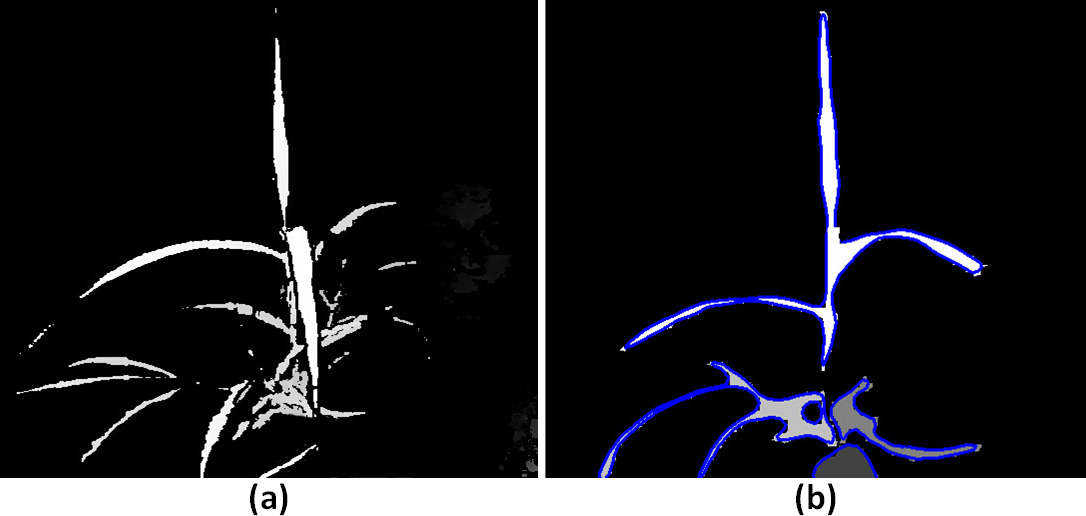
\includegraphics[width=0.48\textwidth]{figs/depth_contour2.jpg}
    \captionof{figure}{(a)Depth image and (b)extracted contour}
    \label{fig:depthimage}
\end{figure}

Figure\ref{fig:depthimage} shows the depth image of a cluster of grass blades and its extracted contour. We just use depth information to mask objects that exceed specified depth to get a blob of blades and then extract edge of the blob. Also canny edge detection can be used to extract contour, however depth value, instead of gray is used to do calculation.

\subsection{Single Blade Partition}

Individual grass blades are partitioned by a particle-flow method\cite{neubert2007approximate}. After getting the contour of grass blades, the center of the contour can be easily calculated. Then the distance between any point on the contour and center point can be measured. Local minimum points of point-distance function imply the intersection points between adjacent blades. Boundary between two intersection points is contour of a single blade. Figure.\ref{fig:partition} shows the partition result projected in 2D plane.

\begin{figure}
    \centering
    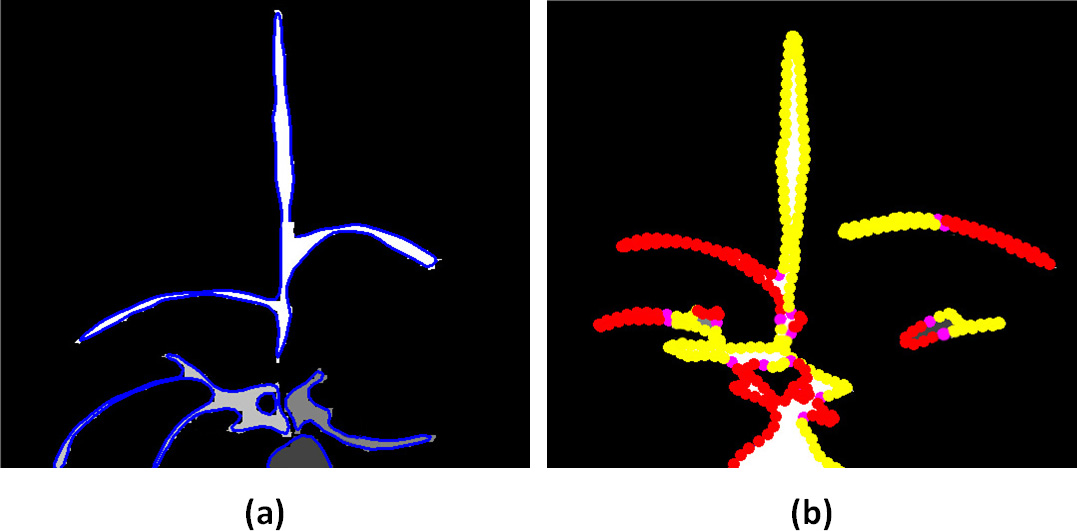
\includegraphics[width=0.48\textwidth]{figs/contour_partition2.jpg}
    \captionof{figure}{Single blade partition: Given the (a)contour of a blade cluster,(b)calculate the center point and use particle-flow method to partition each single blade.}
    \label{fig:partition}
\end{figure}

\subsection{Skeleton and Expansion Width Calculation}
Given the contour of single blade, we could calculate the blade skeleton. According to our observation on plenty kinds of grass blade ,we suppose that captured blade is symmetrical. Then we could calculate skeleton point by matching symmetrical points on contour. Figure.\ref{fig:skeleton} present skeleton calculation according to blade contour. Expansion width for each point of skeleton could also be calculated by symmetrical points' distance.

\begin{figure}
    \centering
    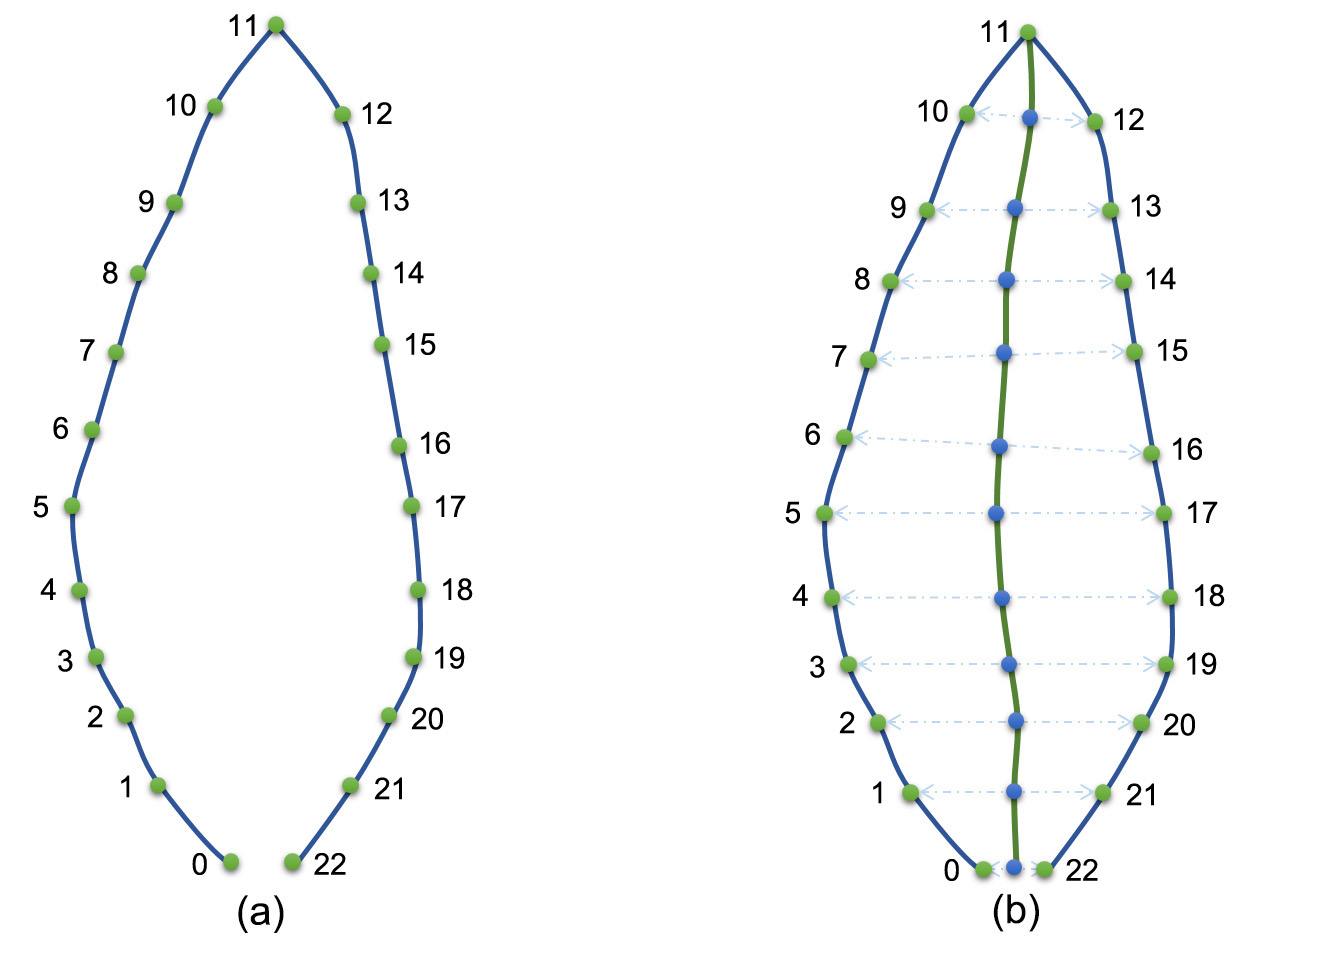
\includegraphics[width=0.45\textwidth]{figs/skeletoncal.jpg}
    \captionof{figure}{Skeleton calculation by match symmetrical points on contour.(a) capture single blade contour points, points index increases from bottom left to bottom right;(b) Matching symmetrical points in the contour.}
    \label{fig:skeleton}
\end{figure}

\subsection{Skeleton Refining}\label{sec:Refining}
Having the blade skeleton calculated from contour, it can't be used in our rendering and simulation system for its large number of vertices. Therefore we come up with a skeleton refining method to simplify our skeleton model. This skeleton refining method is similar to some LOD methods. However most LOD methods are designed for triangle meshes or quad meshes. Our skeleton is represented as a curve and more importantly, we need to take geometry fidelity as well as vertices' movement similarity into account simultaneously while doing simplification. Therefore we design this refining scheme that both geometry and simulation similarities of vertices are important factors in skeleton simplification and fidelity evaluation.\\

In our system, we define any two vertices' movement similarity by the distance between them and their movement trends. For any two vertices, the smaller the distance between them is, the more similar they are. And for any two vertices, we could calculate the distance between them at any time. We could acquire the distance of two vertices every a few millisecond. Then we are able to calculate a series distance data for these two vertices. Variance is usually used to describe data stability. If distance variance is low, it means the distance between two vertices is stable. In another word, this indicate that these two vertices moves synchronously. We tend to merge vertices that moves similarly and keep vertices that have distinct movement features. Assume we acquire $n$ frames every a few milliseconds, $v_{m}^{n}$ is $m$th vertex at $n$th frame, therefore we introduce movement difference of any two vertices as:

\begin{equation}
D(v_{1}, v_{2}) = dis(v_{1}, v_{2})\times \mu + var(v_{1}, v_{2}) \times (1-\mu)
\label{eq:similarityeq}
\end{equation}

\begin{equation}
dis(v_{1}, v_{2}) = \dfrac{\sum_{i = 0}^{n}{d(v_{1}^{i}, v_{2}^{i})}}{n}
\label{eq:distance}
\end{equation}

\begin{equation}
var(v_{1}, v_{2}) = (\dfrac{\sum_{i = 0}^{n}{d(v_{1}^{i}, v_{2}^{i})}^{2}}{n} - \dfrac{(\sum_{i = 0}^{n}{d(v_{1}^{i}, v_{2}^{i})})^{2}}{n})
\label{eq:variance}
\end{equation}

$dis$ function represents distance factor and $var$ function represents variance factor. $\mu$ is proportion factor for distance and variance, which can be set by user.\\

We use an iterative algorithm to complete this skeleton refining process. After skeleton calculation, we manage to obtain array of skeleton vertices. We design a greedy algorithm to iteratively merge two adjacent vertices, based on the assumption that if two vertices are the most similar then they should be adjacent vertices in the array. Because distance factor is an very important part in similarity definition, and closer vertices always get lower score for distance factor. This algorithm is illustrated in Algorithm.\ref{tbl:skeletonrefining}.\\

\floatname{algorithm}{Algorithm}
    \renewcommand{\algorithmicrequire}{\textbf{Input:}}
    \renewcommand{\algorithmicensure}{\textbf{Output:}}

    \begin{algorithm}
        \caption{Skeleton Refining}
        \label{tbl:skeletonrefining}
        \begin{algorithmic}[1]
            \State //SkeletonVertices = Calculated from captured result
            \While{SkeletonVertices.size()  $> m$}
                \State DifferenceArr = $\emptyset$
                \For{$v_{i}$ in SkeletonVertices}
                    \State $d_i = D(v_{i}, v_{i+1})$
                    \State DifferenceArr.add($d_i$)
                \EndFor

                \\
                \State //Search for minimum $d$ in DifferenceArr
                \State $ind$ = DifferenceArr.minimum()
                \State $newV = (v_{i} + v_{i+1}) /2$
                \\
                \State //Delete old vertices
                \State DifferenceArr.delete($ind$)
                \State DifferenceArr.delete($ind+1$)
                \\
                \State //Insert new vertex at position i
                \State DifferenceArr.insert($newV$, $ind$)

            \EndWhile
        \end{algorithmic}
    \end{algorithm}

\begin{figure}
    \centering
    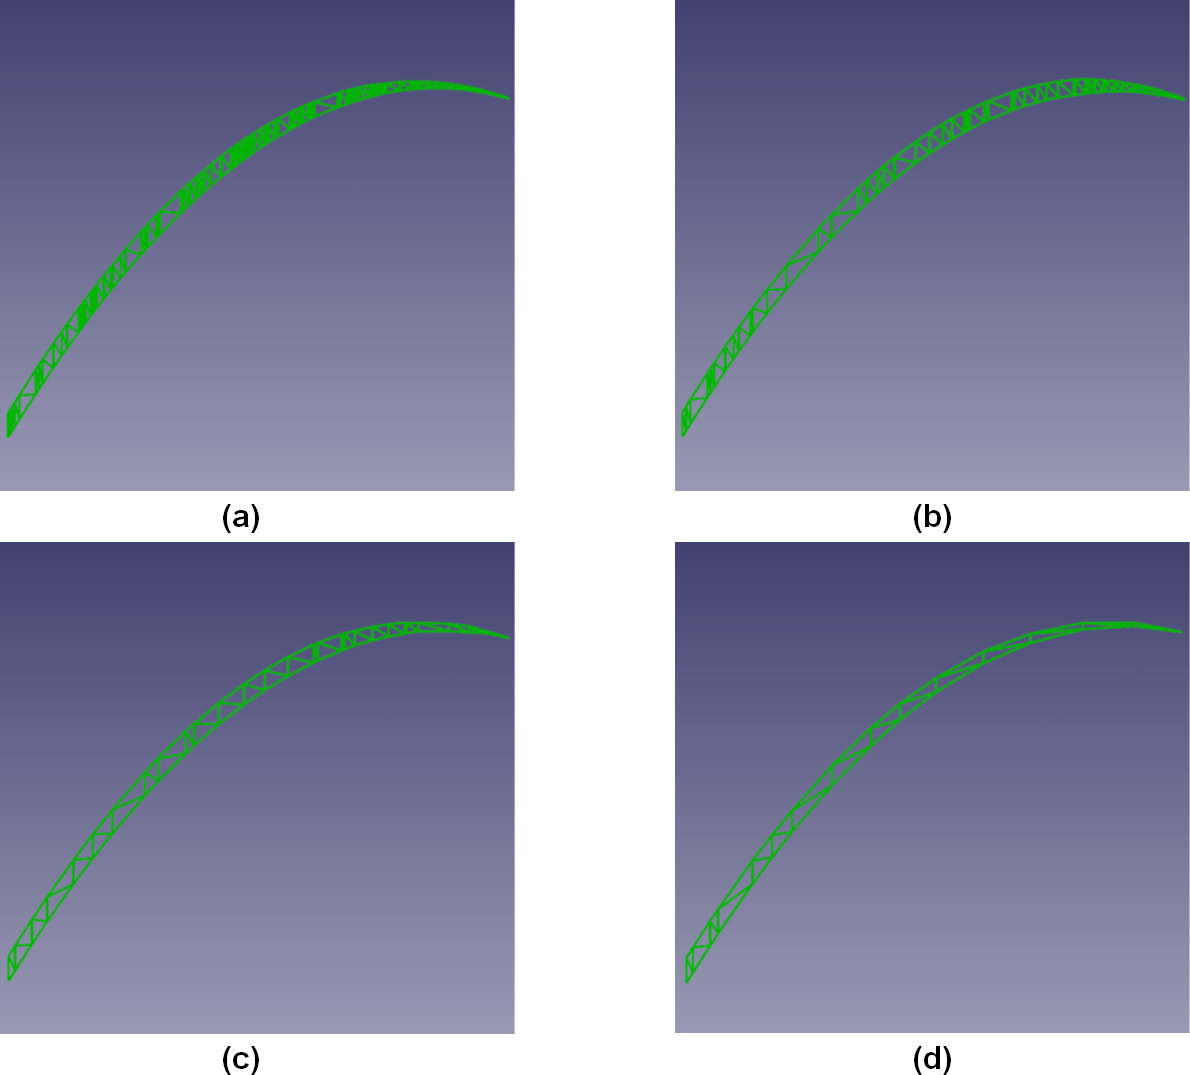
\includegraphics[width=0.48\textwidth]{figs/lod3.jpg}
    \captionof{figure}{Skeleton refining process with a sequence of idealized grass blade skeleton��in the figure this skeleton is expanded as it is done in vertex shader, at first there is (a) blade skeleton with 128 vertices; after different level of skeleton refining, (b) blade skeleton with 64 vertices; (c) blade skeleton with 32 vertices; (d) blade skeleton with 16 vertices.}
    \label{fig:skeletonrefining}
\end{figure}

Figure.\ref{fig:skeletonrefining} illustrates a sequence of grass blade with different refining level. Refining level is set by user according to the performance requirement of application and hardware level.

\subsection{Rendering and Simulation}\label{sec:render}
According to our captured grass model and refining result, we pre-generate a list of grass blades with some random scaling.We divide the whole scene into tiles. Those blades in the patch are randomly located in a square which has the same size of grass tile in the scene. Each tile contains a subset of continuous blades in the patch. For each grass tile, its offset in the patch is calculated by tile's position coordinate in the scene. With this instancing scheme, we are able to reduce memory use from about $4$ GB of $4$ M blades to only $24$ MB of for a patch of $16384$ blades. With this patch, we manage to implement a grassland with rich variance.\\

We draw one line segment as two degenerate triangles and expand each knot of this line segment at runtime according to expansion width captured through depth camera. Figure.\ref{fig:expasion} illustrates this expansion process. We employ Phong shading along with subsurface scattering effect\cite{sousa2007vegetation} in our system. In order to avoid a monotone we use a density map in our system. Figure.\ref{fig:density} illustrated our density map generated with Perlin noise\cite{perlin1985image}. \\

\begin{figure}
    \centering
    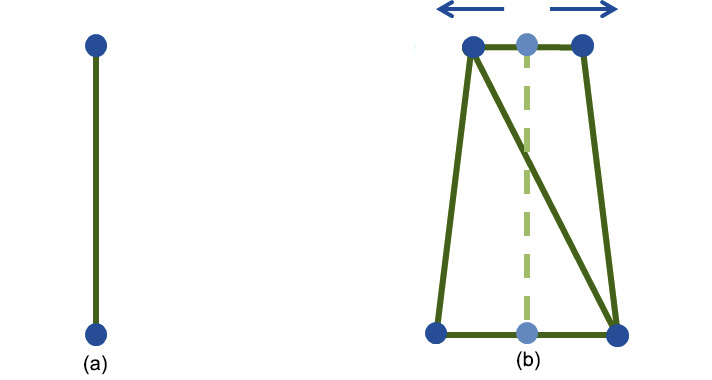
\includegraphics[width=0.48\textwidth]{figs/expansion.jpg}
    \captionof{figure}{Blade skeleton expansion:(a) Simulation blade skeleton presented by overlapping vertices; (b) Expanded triangle model from blade skeleton for rendering; (c) shaded result.}
    \label{fig:expasion}
\end{figure}

\begin{figure}
    \centering
    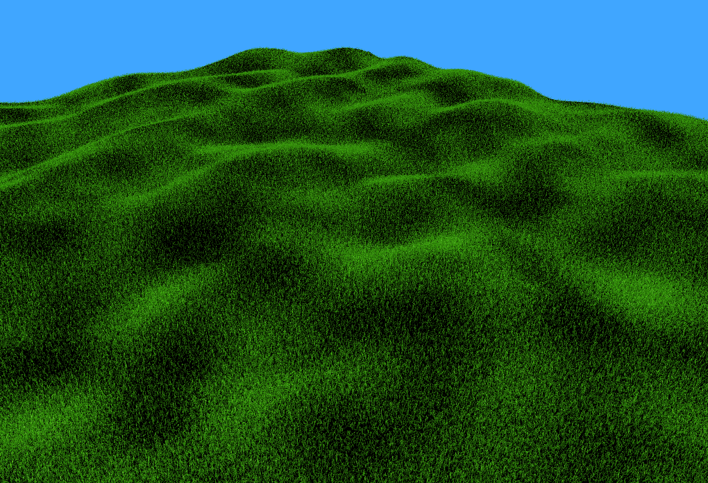
\includegraphics[width=0.48\textwidth]{figs/density.png}
    \captionof{figure}{Density map used in our rendering system.}
    \label{fig:density}
\end{figure}
In our simulation system, $Bullet$ is used to handle collision between ground and other object. We use the simulation method introduced by \cite{han2012real} and tile management scheme introduced by \cite{fan2015simulation}. This simulation scheme is compatible with procedural animation. We are able to simulate millions of grass blades with real-time performance.

\begin{figure*}
    \centering
    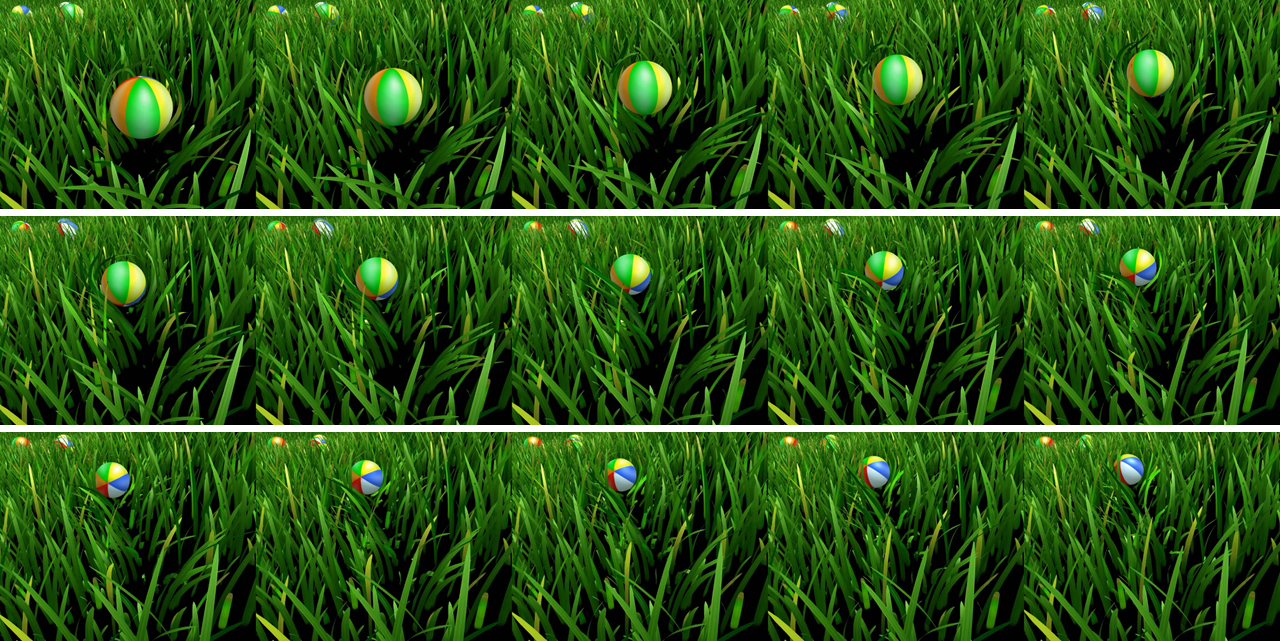
\includegraphics[width=0.98\textwidth]{figs/sim2.jpg}
    \captionof{figure}{Sequence of frames obtained through our rendering and simulation method.}
    \label{fig:simseq}
\end{figure*}


\section{Implementation and Results}
\begin{figure*}
    \centering
    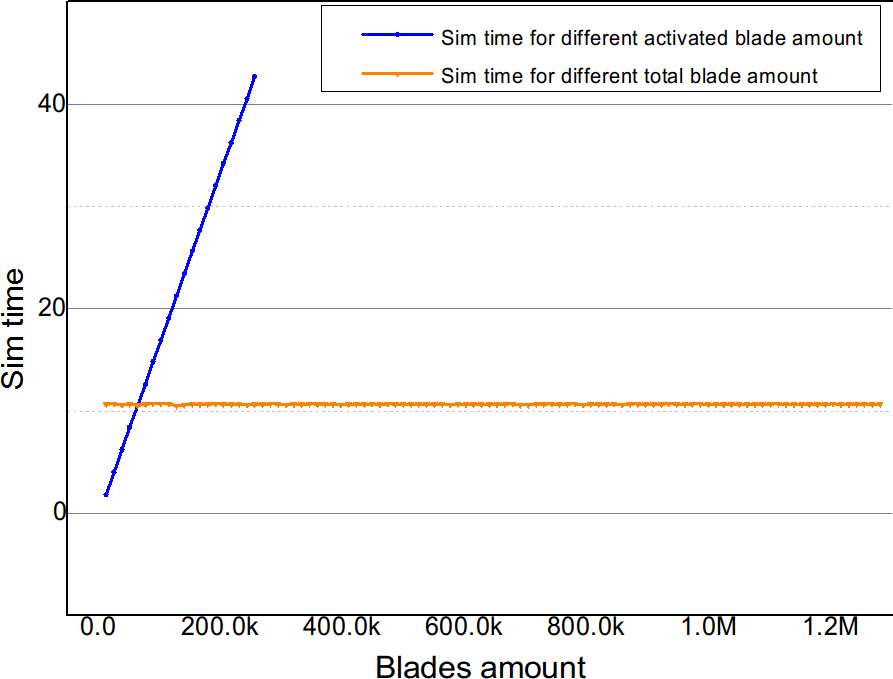
\includegraphics[width=0.8\textwidth, height = 20cm]{figs/results.jpg}
    \captionof{figure}{Experiment results:(a) regular slim and thin grass blade ;(b) blade similar to most leaves, blade edge is quadratic curve like; (c) blade that is slender than the first one, blade edge is still regular (d) bamboo leaf which is thin, its edge is very smooth and flat except for its top and root; (e) leaf with shape variation, it has a very sharp and narrow tip.}
    \label{fig:results}
\end{figure*}

We implemented our system on a PC with Windows 8.1, Intel i5-4460 CPU running at $3.2$ GHz and AMD Radeon R9-270 graphic card. 4 times multi-sampling anti-aliasing is used in all experiments to guarantee satisfactory effect.\\

Instancing rendering is used in our implementation in order to reduce draw call overhead for CPU. Instancing parameters are pre-generated and stored in a structure buffer before rendering. Our rendering scheme is also compatible with different LOD algorithms to at far distance.\\

\subsection{Capture, Rendering and Simulation Results}
Our system is evaluated with a variety of grass blades and leaves that can be used for large scale grassland. Our capture algorithm can capture grass blade, partition single blade contour, calculate expansion width and finish skeleton refining at interactive performance. This provide the possibility for user to capture any appropriate kind of grass or leaves and use it for large scale grassland rendering and simulation. This is especially useful for virtual-reality or augmented-reality applications where quick reconstruction of grassland with specific grass blade type is needed. \\



In Figure.\ref{fig:results}(a) we choose a regular kind of grass which is slim ,thin and common to find everywhere.  In (b) we choose a vine and capture its leaf as grass blade. This blade is like a tree leaf, its blade edge can be described as a quadratic curve. In (c) we choose a cluster of leaves from a shrub. This leaf is longer however its blade edge is still regular and quadratic-curve like. In (d) we choose a cluster of bamboo leaves. Bamboo leave is thin and slim, from the figure we could see that its blade edge is very smooth and flat in the middle and it is hard to be described with simple quadratic curves. In(e) we choose a leaf with variation it the top. It has a very sharp and narrow tip which make it special. Camera captured this feature kept it through our expansion width calculation.\\

\begin{table}[ht]
\begin{center}
 \begin{tabular}{|c|c|c|c|c|}
     \hline
     \textbf{Tiles} & 6 & 14 & 150 & 709 \\
     \hline
     \textbf{Blades}& 384 & 896 & 9600 & 45376 \\
     \hline
     \textbf{Objects} & 1 & 2 & 20 & 128 \\
     \hline
     \textbf{Sim time(ms)} & 0.176 & 0.183 & 0.952 & 4.67 \\
     \hline
     \textbf{Sim time/Blade (ns)} & 0.458 & 0.204 & 0.099 & 0.103 \\
     \hline
 \end{tabular}
 \caption{Simulation time data with different activated tiles, objects.}
 \label{table:frameprofile}
 \end{center}
 \end{table}

We have tested our algorithm to evaluate its rendering and simulation performance. In our system, we need only one draw call to rendering the whole scene, which greatly reduce CPU overhead. We are able to render a scene of $14926$ tiles in $20$ ms, in total there are $955264$ blades and over $29$ million triangles. In table.\ref{table:frameprofile}, profiling data for simulation demonstrates the effectiveness of our system. Simulation time for a single blade decreases with the increase of simulated tiles as listed in the table. This gives the evidence that our system is suitable to solve the high simulation cost problem caused by extremely large grassland.\\

\subsection{Skeleton Refining Evaluation}
For error measurement of meshes, several methods such as the use error metric of average squared distance were used in previous works\cite{garland1997surface}. Our grass blade skeleton is represented as a curve, in order to measure the effectiveness of our skeleton refining algorithm, we use a Hausdorff-Fit method to evaluate the refining result. We intend to measure the "distance" between refined skeleton and the original one before refining, as it is demonstrated in Figure.\ref{fig:distance}. This is very similar to error metric or energy term used in previous methods. Hausdorff distance is usually used to measure how far two subsets of a metric space are from each other\cite{wikihausdorff}. Hausdorff distance is the maximum distance of a set to the nearest point in the other set.

\begin{figure}
    \centering
    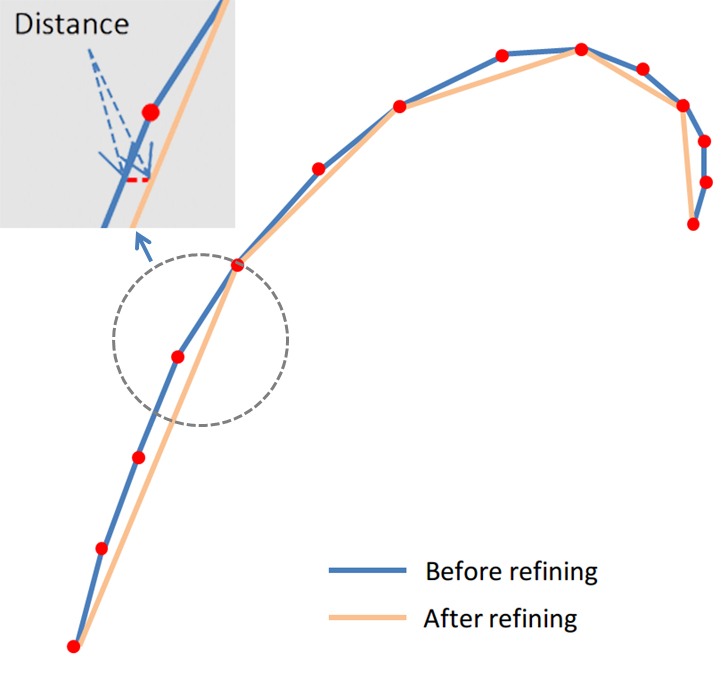
\includegraphics[width=0.4\textwidth]{figs/distance.jpg}
    \captionof{figure}{Distance between refined skeleton and original skeleton calculated from blade contour.}
    \label{fig:distance}
\end{figure}

Hausdorff distance is usually defined as:

\begin{equation}
d_{H}(X,Y) = \max\{\sup_{x \in X }\inf_{y \in Y}d(x,y), \sup_{y \in Y}\inf_{x \in X} d(x,y)\}
\label{eq:hausdorff}
\end{equation}

where $sup$ represents the supremum of the set and $inf$ represents the infimum. $X$, $Y$ are two sets while $x$, $y$ are elements that belong to $X$, $Y$ respectively. In our method, Hausdorff distance is used to measure the similarity of refined skeleton and the original one before refining. However, since the skeleton after refining could be a sub set of the original one, hausdorff distance could become meaningless in that case. Therefore we eliminate the vertices from original skeleton vertex set $\alpha$ if they are also in refined skeleton vertex set $\beta$, let $\alpha' = \alpha - \beta $, then we calculate the hausdorff distance from $\alpha'$ to $\beta$. In this way we actually measure the distance between the culled vertex set and the remained vertex set after refining. Algorithm for our method is demonstrated in algorithm.\ref{tbl:skeletonrefiningeva} where $d_H$ is refined hausdorff distance used in our algorithm.\\

\floatname{algorithm}{Algorithm}
    \begin{algorithm}
        \caption{Skeleton Refining Evaluating}
        \label{tbl:skeletonrefiningeva}
        \begin{algorithmic}[1]
            \State //SkeletonVertices = Calculated from captured result
            \State $\alpha$ = Original skeleton vertex set
            \State $\beta$ = Refined skeleton vertex set
            \For{$v$ in $\alpha$}
                \If {$v$ is $\beta$}
                    \State {Delete $v$ from $\alpha$}
                \EndIf
            \EndFor
            \State
            \State $d_H = MIN$
             \For{$v_1$ in $\alpha$}
                \State $d = MAX$
                \For{$v_2$ in $\beta$}
                    \State $d = min(distance(v_1, v_2), d)$
                \EndFor
                \State $d_H = max(d, d_H)$
             \EndFor

        \end{algorithmic}
    \end{algorithm}

We recorded vertex data from several frames according to our simulation algorithm. Simulation for original skeleton vertices and refined skeleton vertices are conducted at the same time. Then we calculate $d_H$ as in algorithm.\ref{tbl:skeletonrefiningeva} in each frame for the results of different refining methods. For the needs of comparison, we introduces several other schemes used for skeleton refining. Random method selects vertices randomly from original vertex set. Mean method select vertices evenly along the skeleton from the root to the top. only geometry information is used in geometry-based refining algorithm. It iteratively merge vertices with shortest distance of the skeleton. Since grass blade skeleton is represented as a curve, many LOD methods for meshes could degenerate to it eventually. Refining error is represented as $d_H$. From Figure.\ref{fig:evaresults} we could see that our skeleton refining algorithm always gets the lowest error among the methods listed above. Mean method is a intuitive method used in manual grass blade modeling, however it is not a good choice proved with our experiments. Geometry-based simplification is widely used however, it gets higher refining error since it only considers static mesh structure while for dynamic scenes, simulation similarity helps to get a more accurate grass blade model.\\


\begin{figure}
    \centering
    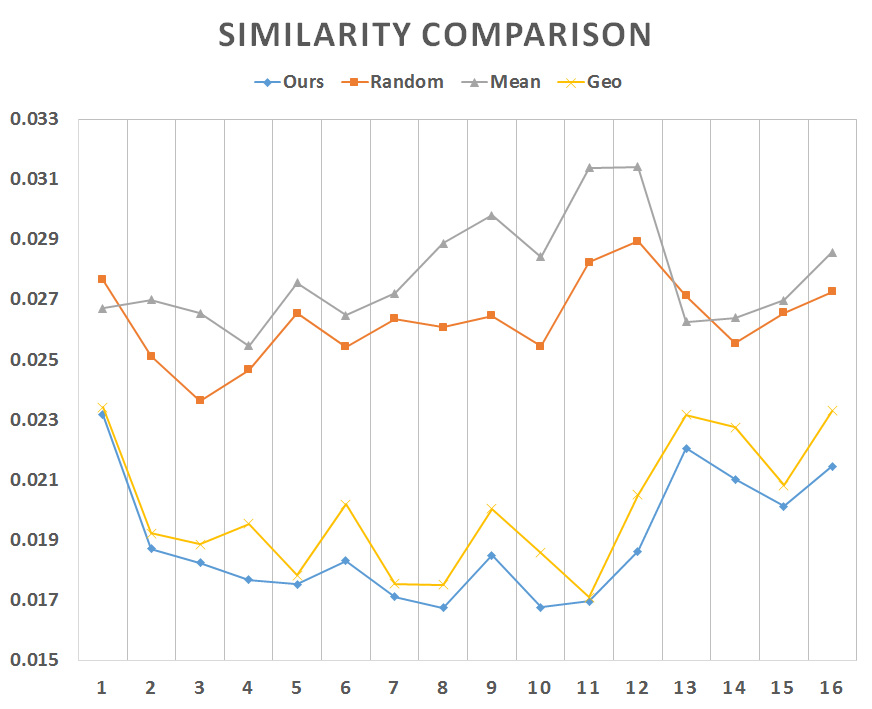
\includegraphics[width=0.48\textwidth]{figs/simcom.jpg}
    \captionof{figure}{Skeleton refining evaluation results: our methods, random method, mean method and geometry-based method. }
    \label{fig:evaresults}
\end{figure}

\textbf{Limitations.} Restricted by vertex amount of grass blade, our method has some limitations. First, small vertex amount is not enough to model jagged blades or leaves. Sharp variation in shape definitely need more vertices to remain such features. However, vertex amount is severely restricted by performance requirements, we need to balance vertex amount and performance at the same time. Meanwhile, due to the structure of grass blade we use in our system, we are not able to handle horizontally curly blades.  Secondly, since we choose to do instancing before rendering and expand grass blade at runtime, moreover our skeleton calculation by matching points will run into difficulties when dealing with asymmetric grass blades or leaves. Thirdly, the center point calculation of a grass blade cluster requires appropriate pose for camera and blade cluster, causing some accuracy problem if the poses are not proper. Fourthly, depth image capture by depth camera only support a maximum resolution of $640\times 480$ pixels, this will cause some problem when we want to capture some small and thin grass blades. Hopefully this problem would be solved with the development of hardware and popularity of depth camera.

\section{Conclusion}
In this paper, we present a framework for capturing grass blade with depth camera, expansion width calculation and skeleton extraction. We utilize a increasingly popular depth camera and take advantage of depth information provided by depth camera to accomplish efficient capturing. We extract a blob of blades according to objects' depth range and calculate its edge to obtain a contour. A particle-flow method is used to partition single blade's contour from a cluster of blades. Based on a single blade's contour, we calculate a skeleton by matching symmetrical vertices on the contour and expansion width for each vertices of the skeleton. A skeleton refining process according to vertices' movement similarity is introduced to reduce skeleton vertex number so that it can be used in the rendering and simulation system with acceptable performance. As for rendering, we adopt a GPU-instanced scheme reduce memory usage. A tile management method is employed to pay simulation cost for those tiles only when needed.\\

Our proposed method concentrate on capturing grass blade shape and refining its structure so that it can be used in the rendering and simulation method for large scale grassland. We are able to a variety of grass blades. We would like to extend our method to handle more complex blade shapes or capture other kind of plants. Furthermore, our method does not handle grass fracture and deformation. Skeleton and expansion width calculation may get incorrect result with such cases. We plan to handle grass fracture in future works and add support for structurally different vegetation.\\

In summary, our work demonstrate how interactive capturing method can be developed to model grass blade and use it in rendering and simulation frameworks. This work can be extended to many fields and inspire other capturing and modeling method for plants and other relative objects.



% if have a single appendix:
%\appendix[Proof of the Zonklar Equations]
% or
%\appendix  % for no appendix heading
% do not use \section anymore after \appendix, only \section*
% is possibly needed

% use appendices with more than one appendix
% then use \section to start each appendix
% you must declare a \section before using any
% \subsection or using \label (\appendices by itself
% starts a section numbered zero.)
%


%\appendices
%\section{Proof of the First Zonklar Equation}
%Appendix one text goes here.
%
%% you can choose not to have a title for an appendix
%% if you want by leaving the argument blank
%\section{}
%Appendix two text goes here.


% use section* for acknowledgment
\ifCLASSOPTIONcompsoc
  % The Computer Society usually uses the plural form
  \section*{Acknowledgments}
\else
  % regular IEEE prefers the singular form
  \section*{Acknowledgment}
\fi

Thank my teammate for helping me with this paper.

% Can use something like this to put references on a page
% by themselves when using endfloat and the captionsoff option.
\ifCLASSOPTIONcaptionsoff
  \newpage
\fi



% trigger a \newpage just before the given reference
% number - used to balance the columns on the last page
% adjust value as needed - may need to be readjusted if
% the document is modified later
%\IEEEtriggeratref{8}
% The "triggered" command can be changed if desired:
%\IEEEtriggercmd{\enlargethispage{-5in}}

% references section

% can use a bibliography generated by BibTeX as a .bbl file
% BibTeX documentation can be easily obtained at:
% http://www.ctan.org/tex-archive/biblio/bibtex/contrib/doc/
% The IEEEtran BibTeX style support page is at:
% http://www.michaelshell.org/tex/ieeetran/bibtex/
%\bibliographystyle{IEEEtran}
% argument is your BibTeX string definitions and bibliography database(s)
%\bibliography{IEEEabrv,../bib/paper}
%
% <OR> manually copy in the resultant .bbl file
% set second argument of \begin to the number of references
% (used to reserve space for the reference number labels box)
%\begin{thebibliography}{1}
%
%\bibitem{IEEEhowto:kopka}
%H.~Kopka and P.~W. Daly, \emph{A Guide to \LaTeX}, 3rd~ed.\hskip 1em plus
%  0.5em minus 0.4em\relax Harlow, England: Addison-Wesley, 1999.
%\bibitem{Reeves1985}
%Reeves W T, Blau R. Approximate and probabilistic algorithms for shading and rendering structured particle systems[C]//ACM Siggraph Computer Graphics. ACM, 1985, 19(3): 313-322.
%
%\end{thebibliography}
\bibliographystyle{IEEEtran}
\bibliography{IEEEabrv,grass}

% biography section
%
% If you have an EPS/PDF photo (graphicx package needed) extra braces are
% needed around the contents of the optional argument to biography to prevent
% the LaTeX parser from getting confused when it sees the complicated
% \includegraphics command within an optional argument. (You could create
% your own custom macro containing the \includegraphics command to make things
% simpler here.)
%\begin{IEEEbiography}[{\includegraphics[width=1in,height=1.25in,clip,keepaspectratio]{mshell}}]{Michael Shell}
% or if you just want to reserve a space for a photo:

\begin{IEEEbiography}[{
\includegraphics[width=1in,height=1.25in,clip,keepaspectratio]{figs/test3.jpg}}]{Zengzhi Fan}
Biography text here.
\end{IEEEbiography}

% if you will not have a photo at all:
\begin{IEEEbiographynophoto}{Bin Sheng}
Biography text here.
\end{IEEEbiographynophoto}

% insert where needed to balance the two columns on the last page with
% biographies
%\newpage


% You can push biographies down or up by placing
% a \vfill before or after them. The appropriate
% use of \vfill depends on what kind of text is
% on the last page and whether or not the columns
% are being equalized.

%\vfill

% Can be used to pull up biographies so that the bottom of the last one
% is flush with the other column.
%\enlargethispage{-5in}



% that's all folks
\end{document}


